\documentclass[a4paper,12pt]{article}

% ---------------------------------------------------------------------------
% Pacotes
% ---------------------------------------------------------------------------
\usepackage[utf8]{inputenc}
\usepackage[T1]{fontenc}
\usepackage[brazilian]{babel}
\usepackage[a4paper,margin=2.5cm]{geometry}
\usepackage{graphicx}
\usepackage{xcolor}
\usepackage{booktabs}
\usepackage{array}
\usepackage{float}
\usepackage{caption}
\usepackage{subcaption}
\usepackage{listings}
\usepackage{tikz}
\usetikzlibrary{calc,arrows.meta}
\usetikzlibrary{shapes.multipart,arrows.meta,positioning,fit,shapes.geometric}
\usepackage{hyperref}
\hypersetup{colorlinks=true, linkcolor=blue!50!black, urlcolor=blue!50!black, citecolor=blue!50!black}

\newcommand{\code}[1]{\texttt{#1}}

\lstdefinestyle{cstyle}{
    language=C,
    basicstyle=\ttfamily\footnotesize,
    keywordstyle=\color{blue!70!black}\bfseries,
    commentstyle=\color{green!40!black}\itshape,
    stringstyle=\color{orange!70!black},
    numbers=left,
    numberstyle=\tiny\color{gray},
    stepnumber=1,
    numbersep=8pt,
    breaklines=true,
    showstringspaces=false,
    frame=single,
    backgroundcolor=\color{gray!5},
    tabsize=4,
}
\lstset{style=cstyle}

\title{\textbf{Pula Plataformas}\\[4pt]
\large Relatório de Implementação\\
Trabalho Final --- Introdução aos Sistemas Embarcados}
\author{Bruno Suxberger Valadares Araújo --- matrícula 231012728 \\
Pedro Araujo Cordeiro Viana --- matrícula 202067452}
\date{\today}

\begin{document}

\maketitle

\begin{abstract}
Este relatório descreve a implementação do \emph{Pula Plataformas}, jogo digital
desenvolvido para a placa DE1-SoC como trabalho final da disciplina de
Introdução aos Sistemas Embarcados. O jogo é um \emph{platformer} vertical
(estilo \emph{Doodle Jump}) em que o personagem sobe pulando entre plataformas
de gelo geradas proceduralmente, desviando de um vilão-nave que patrulha o
topo da tela e atira projéteis que podem ser refletidos de volta por meio de
uma mecânica de \emph{parry}. O documento cobre como compilar e executar o
código, o funcionamento do jogo, as entradas e saídas utilizadas, a estrutura
do código modelada em UML, o pipeline gráfico, o sistema de pontuação e
recordes, e as principais dificuldades encontradas durante o desenvolvimento.
\end{abstract}

\tableofcontents

% =============================================================================
\section{Introdução}
% =============================================================================

O trabalho consiste em um jogo de plataforma para a DE1-SoC, utilizando o
vídeo VGA, os mostradores de 7 segmentos e os periféricos de entrada da placa
(chaves e botões). Diferente do jogo de deslocamento horizontal estilo
``Mário'' sugerido no enunciado original, optou-se por um jogo de escalada
vertical infinita: o personagem (Kirby) sobe pulando de plataforma em
plataforma, tentando alcançar uma pontuação máxima antes que suas vidas
acabem, enquanto enfrenta um vilão que atira nele do topo da tela.

O código-fonte principal está em \code{pula\_plat.c} e é organizado em torno de
um laço de jogo clássico (leitura de entrada, atualização de estado,
renderização), com suporte a três alvos de compilação diferentes por meio de
\emph{flags} do pré-processador, descritos na Seção~\ref{sec:compilar}.

% =============================================================================
\section{Como compilar e executar}
\label{sec:compilar}
% =============================================================================

O jogo foi escrito para compilar em três ambientes diferentes, selecionados
por \emph{flags} de compilação, sem alterar a lógica do jogo:

\begin{itemize}
    \item \textbf{DE1-SoC real} (\code{-DDE1\_SOC}): acessa os endereços de
    memória da VGA, dos LEDs, das chaves e dos botões diretamente via
    \code{/dev/mem}, exigindo execução como \emph{root}.
    \item \textbf{CPUlator}, sem nenhuma \emph{flag}: os mesmos endereços de
    memória usados na DE1-SoC real são acessíveis diretamente dentro do
    simulador, sem necessidade de \code{mmap}.
    \item \textbf{SDL\_SIM} (\code{-DSDL\_SIM}): substitui a VGA por uma janela
    SDL2 e as chaves/botões pelo teclado, permitindo testar o jogo em um PC
    comum (Windows, via MSYS2), sem precisar da placa nem do simulador.
\end{itemize}

\subsection{Simulação do CPUlator ao MSYS2}

No início do desenvolvimento, o projeto foi testado exclusivamente no
\textbf{CPUlator} (\url{https://cpulator.01xz.net}), um simulador da DE1-SoC
que roda inteiramente no navegador. Ele é útil por não exigir acesso à placa
física, mas impõe limitações sérias para um projeto que cresce em
complexidade: aceita apenas um único arquivo \code{.c} colado no editor (sem
suporte a múltiplos arquivos ou \code{\#include} de arquivos locais), não
possui um sistema de arquivos persistente entre execuções (impossibilitando,
por exemplo, salvar o arquivo de recordes descrito na
Seção~\ref{sec:pontuacao}), e o ciclo de teste --- editar, colar no navegador,
rodar --- é sensivelmente mais lento do que compilar e rodar localmente.

À medida que o projeto ganhou sprites (múltiplos arquivos \code{.h} gerados
separadamente), um vilão, um sistema de recordes persistente e um laço de
testes muito mais iterativo, tornou-se preferível desenvolver e testar
localmente usando o \textbf{MSYS2}. MSYS2 é uma distribuição de software para
Windows que fornece um ambiente do tipo Unix (terminal, utilitários
\emph{shell}) e um gerenciador de pacotes (\code{pacman}) com \emph{toolchains}
pré-compiladas --- em particular o MinGW-w64, uma versão do GCC que gera
executáveis nativos do Windows (\code{.exe}) em vez de exigir uma máquina
virtual Linux ou o WSL. Combinado com a biblioteca SDL2 (que abstrai janela,
teclado e \emph{framebuffer}), isso permite compilar e rodar o jogo
localmente com um laço de desenvolvimento rápido, mantendo o mesmo código
C que roda na placa.

O arquivo \code{pula\_plat.c} usa \code{\#include} para os \emph{headers} de
sprite (ver Seção~\ref{sec:graficos}), o que o CPUlator não aceita. Por isso,
o repositório do projeto mantém um script auxiliar, \code{tools/build\_cpulator.py}, que
gera uma versão de \code{pula\_plat.c} com todos os \code{\#include} locais
``inlinados'' em um único arquivo (\code{pula\_plat\_cpulator.c}), apenas para
os casos em que ainda seja necessário validar no simulador. Esse arquivo é
puramente derivado --- não é editado diretamente, e é regerado a partir de
\code{pula\_plat.c} sempre que necessário; o desenvolvimento e os testes do
dia a dia acontecem no MSYS2.

\subsection{Compilando com MSYS2 (SDL2) --- fluxo usado no desenvolvimento}

\begin{enumerate}
    \item Instalar o \href{https://www.msys2.org/}{MSYS2} e abrir o terminal
    \textbf{``MSYS2 MinGW 64-bit''} (não o ``MSYS2 MSYS'' genérico, que não
    gera binários nativos do Windows).
    \item Instalar o compilador e a SDL2:
\begin{lstlisting}[language=bash,numbers=none]
pacman -S mingw-w64-x86_64-gcc mingw-w64-x86_64-SDL2
\end{lstlisting}
    \item Compilar:
\begin{lstlisting}[language=bash,numbers=none]
gcc -DSDL_SIM pula_plat.c -o jogo.exe -lSDL2 -lm
\end{lstlisting}
    \item Executar (de dentro do mesmo terminal, que já tem o \code{SDL2.dll}
    no \code{PATH}):
\begin{lstlisting}[language=bash,numbers=none]
./jogo.exe
\end{lstlisting}
    Para rodar fora desse terminal, basta copiar \code{SDL2.dll} para a mesma pasta do executável.
\end{enumerate}

Os controles no modo SDL são o teclado: setas ou WASD para movimento
horizontal, espaço ou seta para cima para pular, e \emph{shift} para o
\emph{parry}. Pontuação e vidas aparecem no título da janela, já que não há
mostrador de 7 segmentos nem LEDs de verdade nesse modo.

\subsection{Compilando para a DE1-SoC real}

\begin{lstlisting}[language=bash,numbers=none]
gcc -DDE1_SOC pula_plat.c -o jogo -lm
sudo ./jogo    # precisa de root para acessar /dev/mem
\end{lstlisting}

\subsection{Execução na placa DE1-SoC}

Para validar o funcionamento fora do CPUlator, o jogo também foi executado
diretamente na placa DE1-SoC real, com o VGA da placa exibindo a tela do
jogo e os LEDs/HEX refletindo o estado das vidas e da pontuação (ver
\texttt{atualiza\_leds} e \texttt{atualiza\_display}). A Figura~\ref{fig:de1soc-fotos}
mostra a placa em funcionamento em diferentes momentos da partida.

\begin{figure}[H]
    \centering
    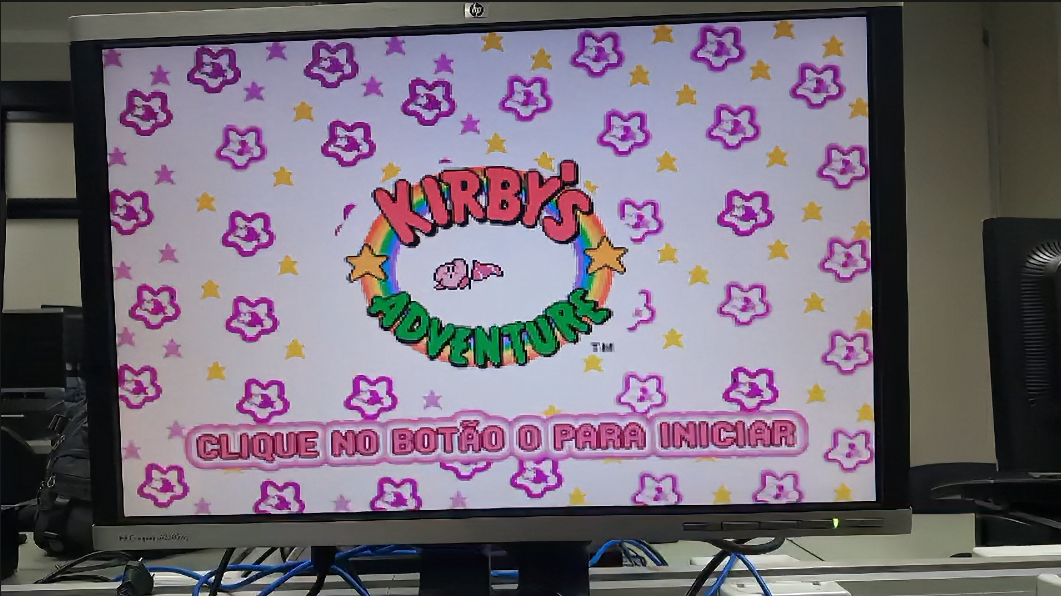
\includegraphics[width=0.7\textwidth]{figuras/de1soc_tela_inicio.png}
    \caption{Tela de início}
    \label{fig:de1soc-inicio}
\end{figure}

\begin{figure}[H]
    \centering
    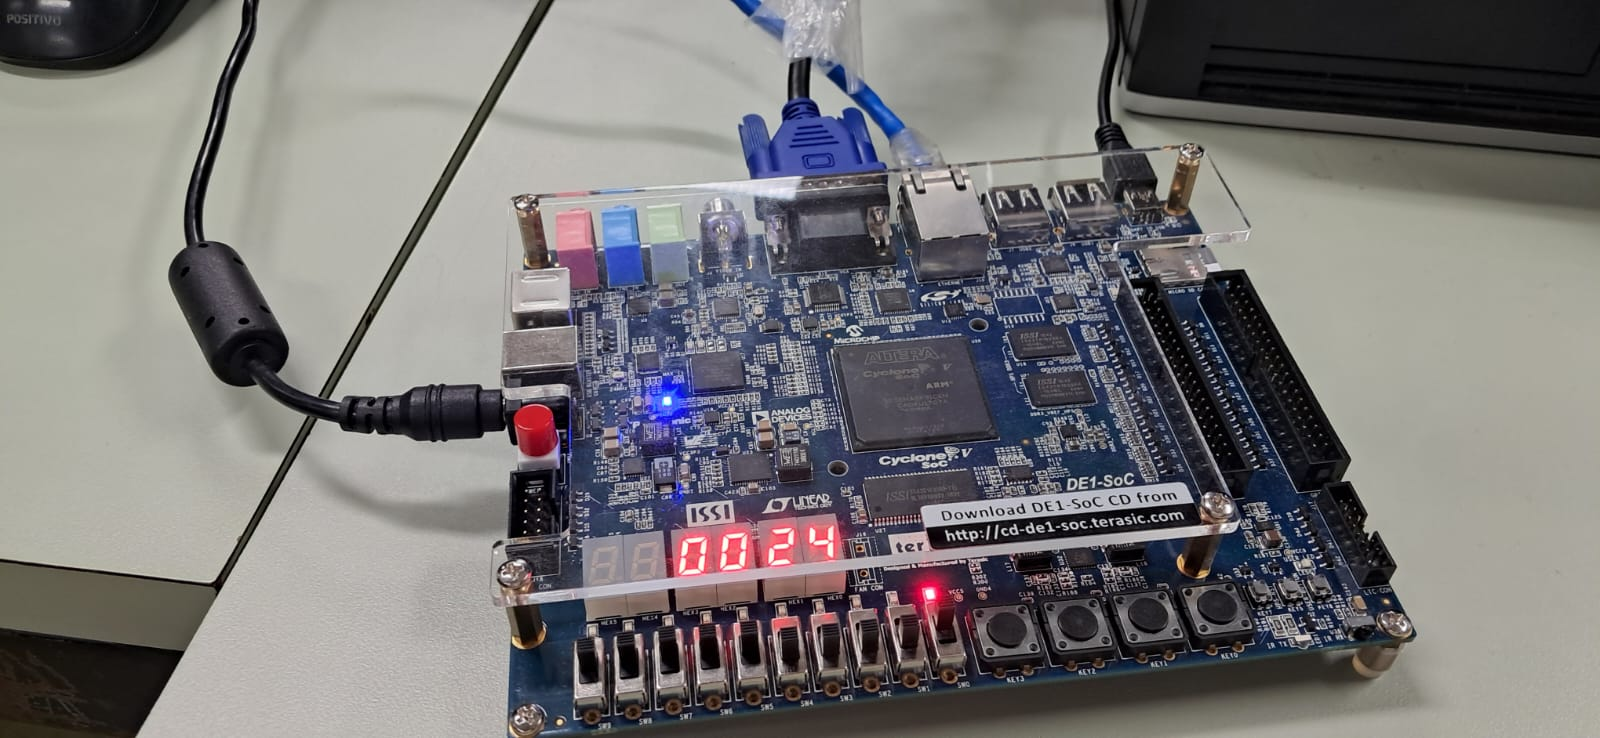
\includegraphics[width=1\textwidth]{figuras/de1soc.jpeg}
    \caption{LEDs e display de 7 segmentos mostrando vidas/pontos}
    \label{fig:de1soc-fotos}
\end{figure}

\begin{figure}[H]
    \centering
    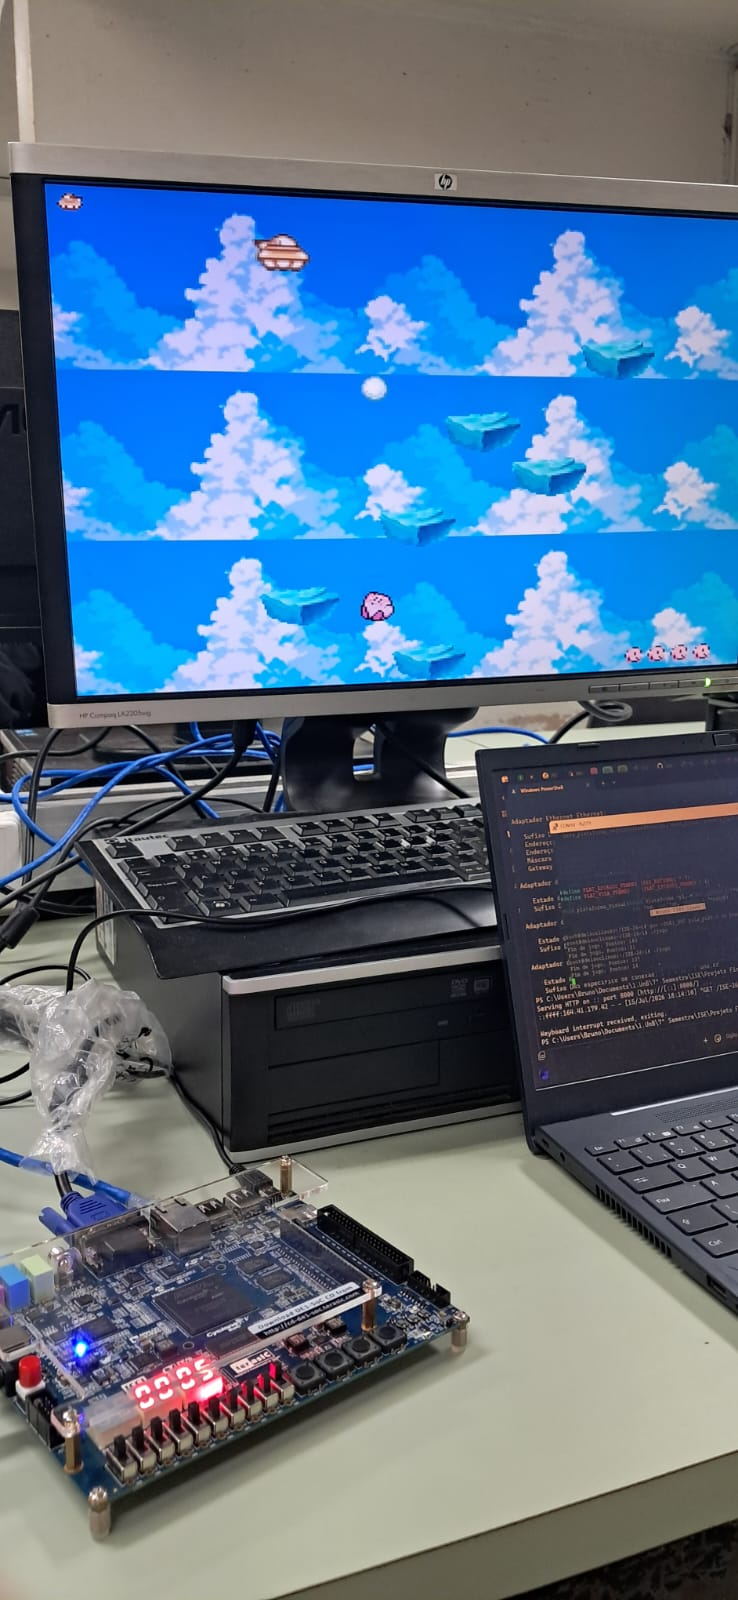
\includegraphics[width=0.4\textwidth]{figuras/jogo_rodando.jpeg}
    \caption{Partida em andamento}
    \label{fig:de1soc-jogando}
\end{figure}



% =============================================================================
\section{Funcionamento do jogo}
% =============================================================================

O jogo segue a estrutura clássica de laço de jogo (\emph{game loop}),
implementada na função \code{main}, com uma máquina de estados simples por
cima controlando qual tela é mostrada:

\begin{lstlisting}[caption={Laço principal, em \code{pula\_plat.c}}]
while (programa_rodando) {
    ler_entrada(&esquerda, &direita, &pular, &parry);
    switch (estado_jogo) {
    case ESTADO_INICIO:    renderiza_tela_inicio();   break;
    case ESTADO_JOGANDO:   atualiza_estado(...); atualiza_vilao();
                           atualiza_projetil(...); atualiza_derretimento();
                           renderiza_cena(...);        break;
    case ESTADO_GAME_OVER: renderiza_tela_game_over(); break;
    case ESTADO_VITORIA:   renderiza_cena(...);        break;
    }
}
\end{lstlisting}

A Figura~\ref{fig:estados} mostra essa máquina de estados. O diagrama de
estados interno do vilão é discutido junto com a Seção~\ref{sec:uml}.

\begin{itemize}
    \item \textbf{Tela de início}: mostra uma animação simples do personagem;
    apertar o botão de mover para a direita começa uma nova partida.
    \item \textbf{Jogando}: o núcleo do jogo --- física de pulo, geração de
    plataformas, vilão e projétil, pontuação.
    \item \textbf{Game over}: mostrado quando as vidas do personagem chegam a
    zero; permite reiniciar ou sair.
    \item \textbf{Vitória}: mostrado ao alcançar a pontuação máxima; congela a
    cena com o personagem em pose de campeão.
\end{itemize}

\textbf{Mecânicas principais:}

\begin{itemize}
    \item \textbf{Física do pulo}: gravidade e velocidade em ponto fixo
    24.8 (1~pixel = 256), atualizadas a cada quadro. A colisão com uma
    plataforma só é testada durante a descida do pulo, fazendo o personagem
    pousar exatamente sobre ela.
    \item \textbf{Geração procedural de plataformas}: a cada plataforma nova,
    sorteia-se uma altura e um deslocamento horizontal compatíveis com o
    alcance físico do pulo (função \code{alcance\_horizontal()}), garantindo
    que todo salto gerado seja sempre alcançável. Um conjunto fixo de 6
    plataformas é reaproveitado indefinidamente: uma plataforma só é
    reciclada (reposicionada acima) depois que o jogador realmente pousou em
    pelo menos 3 plataformas mais recentes que ela, nunca enquanto ainda
    pode ser necessária como apoio.
    \item \textbf{Derretimento}: toda plataforma dura 12 segundos desde que é
    gerada, percorrendo 4 estágios visuais (gelo íntegro e 3 estágios de
    derretimento cada vez menores) antes de sumir e ser reciclada.
    \item \textbf{Câmera}: a câmera só sobe (o jogador nunca desce de tela),
    empurrando o cenário para baixo conforme o personagem sobe além de um
    limiar próximo ao topo da tela.
    \item \textbf{Vilão e projétil}: uma nave patrulha o topo da tela e atira
    periodicamente um projétil mirado na posição do personagem. Segurando o
    botão de \emph{parry} no instante do impacto, o projétil é refletido de
    volta (reto ou na diagonal, conforme a direção escolhida) e pode acertar
    o próprio vilão, tirando uma de suas vidas.
    \item \textbf{Vidas e renascimento}: levar um tiro ou cair da tela custa
    uma vida; o personagem sempre renasce em cima de uma plataforma já
    gerada (nunca em um ponto arbitrário sem chão embaixo).
\end{itemize}

\begin{figure}[H]
    \centering
    \begin{tikzpicture}[
        state/.style={draw, rounded corners, minimum width=2.6cm, minimum height=1cm, align=center, font=\small},
        >=Stealth
    ]
        \node[state] (inicio) {Início};
        \node[state, right=3.2cm of inicio] (jogando) {Jogando};
        \node[state, above right=1.4cm and 3.2cm of jogando] (vitoria) {Vitória};
        \node[state, below right=1.4cm and 3.2cm of jogando] (gameover) {Game Over};

        \draw[->] (inicio) -- node[above,font=\scriptsize]{botão direita} (jogando);
        \draw[->] (jogando) -- node[above,sloped,font=\scriptsize]{pontos $\geq$ máximo} (vitoria);
        \draw[->] (jogando) -- node[below,sloped,font=\scriptsize]{vidas = 0} (gameover);
        \draw[->] (vitoria) to[out=180,in=90] node[right,font=\scriptsize]{botão 1 (retry)} (jogando);
        \draw[->] (gameover) to[out=180,in=-90] node[right,font=\scriptsize]{botão 1 (retry)} (jogando);
    \end{tikzpicture}
    \caption{Máquina de estados do jogo (\code{EstadoJogo}).}
    \label{fig:estados}
\end{figure}

% =============================================================================
\section{Entradas e saídas}
% =============================================================================

\begin{table}[H]
    \centering
    \small
    \begin{tabular}{@{}p{4.2cm}p{7.5cm}c@{}}
        \toprule
        \textbf{Periférico} & \textbf{Uso no jogo} & \textbf{Status} \\
        \midrule
        Vídeo VGA (obrigatório) & Renderização do cenário, plataformas e personagem & Implementado \\
        Displays de 7 segmentos (obrigatório) & Exibição da pontuação & Implementado \\
        LEDs & Exibição do número de vidas restantes & Implementado \\
        Chaves (SW) & Chave 0 = pulo & Implementado \\
        Botões (KEY) & Botões 0/1 = movimento horizontal; botão 2 = \emph{parry} (reflete o projétil); também usados nas telas de início/\emph{game over} & Implementado \\
        \bottomrule
    \end{tabular}
    \caption{Periféricos de entrada/saída da DE1-SoC utilizados pelo jogo.}
\end{table}

No modo \code{SDL\_SIM} (usado para desenvolvimento no PC), o teclado substitui
chaves e botões:

\begin{table}[H]
    \centering
    \small
    \begin{tabular}{@{}ll@{}}
        \toprule
        \textbf{Entrada real (DE1-SoC)} & \textbf{Tecla equivalente (SDL\_SIM)} \\
        \midrule
        Botão 0 / Botão 1 (mover) & Setas esquerda/direita ou A/D \\
        Chave 0 (pular) & Espaço ou seta para cima \\
        Botão 2 (\emph{parry}) & Shift \\
        \bottomrule
    \end{tabular}
    \caption{Mapeamento de teclado no modo SDL\_SIM.}
\end{table}

\textbf{Saídas do jogo:}
\begin{itemize}
    \item \textbf{VGA}: cenário (nuvens de fundo, que mudam de nível a cada 25
    plataformas geradas), plataformas, personagem, vilão, projétil e telas de
    início/\emph{game over}, todos desenhados via \emph{double buffering}
    (Seção~\ref{sec:graficos}).
    \item \textbf{Displays de 7 segmentos}: pontuação atual, em 4 dígitos.
    \item \textbf{LEDs}: uma quantidade de LEDs acesos igual ao número de
    vidas restantes do personagem.
\end{itemize}

% =============================================================================
\section{Estrutura do código (UML)}
\label{sec:uml}
% =============================================================================

O jogo é implementado em C, sem orientação a objetos; ainda assim, os
principais dados do jogo são organizados em \code{struct}s (\code{Player},
\code{Plataforma}, \code{Vilao}, \code{Projetil}, \code{Recordes}), cada uma
associada a um grupo de funções que operam sobre ela --- o mesmo papel que
atributos e métodos cumprem em uma classe. A Figura~\ref{fig:classes}
apresenta essa estrutura como um diagrama de classes simplificado, seguindo a
notação de Wolf (retângulo dividido em nome / atributos / operações).

\begin{figure}[H]
    \centering
    \resizebox{0.75\textwidth}{!}{%
    \begin{tikzpicture}[
        umlclass/.style={
            rectangle split, rectangle split parts=3, draw=black, thick,
            align=left,
            text width=4.4cm, font=\scriptsize, inner sep=5pt,
            rectangle split part fill={blue!8, white, white}
        }
    ]

    \node[umlclass] (jogo) at (2,22) {
        \centering\textbf{Jogo (main)}
        \nodepart{second}
        \begin{tabular}[t]{@{}l@{}}
        estado\_jogo: EstadoJogo\\
        camera\_y: int\\
        frames\_partida: int
        \end{tabular}
        \nodepart{third}
        \begin{tabular}[t]{@{}l@{}}
        main()\\
        ler\_entrada()\\
        atualiza\_estado()\\
        renderiza\_cena()
        \end{tabular}
    };

    \node[umlclass] (recordes) at (10,17.3) {
        \centering\textbf{Recordes}
        \nodepart{second}
        \begin{tabular}[t]{@{}l@{}}
        maior\_pontuacao: int\\
        pontos\_min\_chefe: int\\
        tempo\_min\_vitoria\_frames: int
        \end{tabular}
        \nodepart{third}
        \begin{tabular}[t]{@{}l@{}}
        carrega\_recordes()\\
        salva\_recordes()\\
        registra\_recorde\_*()\\
        desenha\_recordes()
        \end{tabular}
    };

    \node[umlclass] (vilao) at (2,17) {
        \centering\textbf{Vilao}
        \nodepart{second}
        \begin{tabular}[t]{@{}l@{}}
        x: int\\
        dir: int\\
        vidas: int\\
        cooldown\_tiro: int\\
        estado: EstadoVilao\\
        timer: int
        \end{tabular}
        \nodepart{third}
        \begin{tabular}[t]{@{}l@{}}
        atualiza\_vilao()\\
        dispara\_projetil()\\
        desenha\_vilao()
        \end{tabular}
    };

    \node[umlclass] (projetil) at (2,11) {
        \centering\textbf{Projetil}
        \nodepart{second}
        \begin{tabular}[t]{@{}l@{}}
        ativo: int\\
        refletido: int\\
        x, y: int\\
        vx, vy: int
        \end{tabular}
        \nodepart{third}
        \begin{tabular}[t]{@{}l@{}}
        atualiza\_projetil()\\
        desenha\_projetil()
        \end{tabular}
    };

    \node[umlclass] (player) at (2,5.3) {
        \centering\textbf{Player (Kirby)}
        \nodepart{second}
        \begin{tabular}[t]{@{}l@{}}
        x, y: int (24.8 fixo)\\
        vy: int\\
        w, h: int\\
        vidas: int\\
        pontos: int
        \end{tabular}
        \nodepart{third}
        \begin{tabular}[t]{@{}l@{}}
        atualiza\_estado()\\
        desenha\_kirby()\\
        renderiza\_cena()
        \end{tabular}
    };

    \node[umlclass] (plataforma) at (2,-1.5) {
        \centering\textbf{Plataforma}
        \nodepart{second}
        \begin{tabular}[t]{@{}l@{}}
        x, y, w, h: int\\
        melt\_timer: int
        \end{tabular}
        \nodepart{third}
        \begin{tabular}[t]{@{}l@{}}
        gera\_plataforma\_seguinte()\\
        atualiza\_derretimento()\\
        plataforma\_visual()\\
        recicla\_plataformas()\\
        garante\_plataformas\_acima()
        \end{tabular}
    };

    % associações de agregação (losango vazio do lado do "todo" = Jogo)
    \draw[-{Diamond[open]}] (jogo.south) -- node[pos=0.5,right,font=\tiny]{1} (vilao.north);
    \draw[-{Diamond[open]}] (jogo.east) .. controls +(2,-1) and +(0,2) .. node[pos=0.6,above,font=\tiny]{1} (recordes.north);
    \draw[-{Diamond[open]}] (jogo.west) .. controls +(-3,-2) and +(-3,4) .. node[pos=0.5,left,font=\tiny]{0..1} (projetil.west);
    \draw[-{Diamond[open]}] (jogo.west) .. controls +(-5,-4) and +(-5,6) .. node[pos=0.5,left,font=\tiny]{1} (player.west);
    \draw[-{Diamond[open]}] (jogo.west) .. controls +(-7,-8) and +(-7,8) .. node[pos=0.5,left,font=\tiny]{6} (plataforma.west);

    % demais associações
    \draw[->,dashed] (vilao.south) -- node[midway,right,font=\tiny]{cria} node[pos=0.05,left,font=\tiny]{0..1} (projetil.north);
    \draw[-] (projetil.south) -- node[midway,right,font=\tiny]{colide / reflete} node[pos=0.05,left,font=\tiny]{0..1} node[pos=0.95,left,font=\tiny]{1} (player.north);
    \draw[-] (player.south) -- node[midway,right,font=\tiny]{colide com} node[pos=0.05,left,font=\tiny]{1} node[pos=0.95,left,font=\tiny]{6} (plataforma.north);

    \end{tikzpicture}%
    }
    \caption{Diagrama de classes simplificado. Losangos indicam agregação
    (o objeto ``todo'' controla o ciclo de vida das partes); as demais linhas
    são associações. \code{Jogo} representa o laço principal em \code{main()}
    e as funções de nível global do arquivo.}
    \label{fig:classes}
\end{figure}


\subsection{Diagrama de estados do vilão}

Além da máquina de estados do jogo (Figura~\ref{fig:estados}), o vilão
(\code{Vilao}) tem sua própria máquina de estados interna, mostrada na
Figura~\ref{fig:estados-vilao}: ele alterna entre patrulhar/atirar
(\code{NORMAL}), ficar atordoado por 2 segundos após ser atingido
(\code{ATINGIDO}), explodir por mais 2 segundos quando perde a última vida
(\code{EXPLODINDO}) e finalmente desaparecer pelo resto da partida
(\code{MORTO}).

\begin{figure}[H]
    \centering
    \begin{tikzpicture}[
        state/.style={draw, rounded corners, minimum width=2.6cm, minimum height=0.9cm, align=center, font=\small},
        >=Stealth
    ]
        \node[state] (normal) {Normal};
        \node[state, right=3cm of normal] (atingido) {Atingido};
        \node[state, below=1.4cm of atingido] (explodindo) {Explodindo};
        \node[state, below=1.4cm of normal] (morto) {Morto};

        \draw[->] (normal) -- node[above,font=\scriptsize]{tiro refletido acerta} (atingido);
        \draw[->] (atingido) to[out=90,in=90] node[above,font=\scriptsize]{timer = 0, vidas $>$ 0} (normal);
        \draw[->] (atingido) -- node[right,font=\scriptsize]{timer = 0, vidas = 0} (explodindo);
        \draw[->] (explodindo) -- node[above,font=\scriptsize]{timer = 0} (morto);
    \end{tikzpicture}
    \caption{Máquina de estados do vilão (\code{EstadoVilao}).}
    \label{fig:estados-vilao}
\end{figure}

\subsection{Diagrama de sequência: parry e reflexo do projétil}

A Figura~\ref{fig:sequencia} ilustra a interação mais original do jogo: o
jogador reflete de volta o projétil do vilão segurando o \emph{parry} no
instante certo, e o projétil refletido pode, por sua vez, acertar o vilão.

\begin{figure}[H]
\centering
\begin{tikzpicture}[
    >=Stealth,
    font=\small,
    every node/.style={font=\small}
]

%------------------------------------------------
% Atores
%------------------------------------------------
\foreach \x/\nome/\txt in {
0/jogador/{:Jogador},
4/kirby/{:Kirby},
8/projetil/{:Projétil},
12/vilao/{:Vilão}}
{
    \node[draw,minimum width=2.4cm,minimum height=0.8cm] (\nome) at (\x,0) {\txt};
    \draw[dashed] (\nome.south) -- ++(0,-9);
}

%------------------------------------------------
% Mensagens
%------------------------------------------------

% jogador -> kirby
\draw[->]
($(jogador.south)+(0,-1.0)$) --
node[above]{\scriptsize segura parry}
($(kirby.south)+(0,-1.0)$);

% projetil -> kirby
\draw[->]
($(projetil.south)+(0,-2.2)$) --
node[above]{\scriptsize colide (indo)}
($(kirby.south)+(0,-2.2)$);

% kirby -> projetil
\draw[->]
($(kirby.south)+(0,-3.5)$) --
node[above]{\scriptsize reflete (refletido = 1)}
($(projetil.south)+(0,-3.5)$);

% movimento
\node at ($(projetil.south)+(1.8,-5.0)$)
{\scriptsize move em linha reta};

% projetil -> vilao
\draw[->]
($(projetil.south)+(0,-6.3)$) --
node[above]{\scriptsize colide (voltando)}
($(vilao.south)+(0,-6.3)$);

% autochamada
\draw[->]
($(vilao.south)+(0,-7.6)$)
to[out=210,in=150,looseness=8]
node[left]{\scriptsize vidas--}
($(vilao.south)+(0,-7.6)$);

\end{tikzpicture}

\caption{Diagrama de sequência simplificado da mecânica de \emph{parry}
(função \code{atualiza\_projetil()}).}
\label{fig:sequencia}
\end{figure}

\subsection{Principais módulos do arquivo}

\begin{itemize}
    \item \textbf{Física e colisão} (\code{atualiza\_estado}, \code{alcance\_horizontal}):
    gravidade, pulo, colisão com plataformas, pontuação, renascimento.
    \item \textbf{Geração de plataformas} (\code{gera\_plataforma\_seguinte},
    \code{sorteia\_dy}, \code{recicla\_plataformas}, \code{garante\_plataformas\_acima}):
    geração procedural compatível com o alcance do pulo, reciclagem contínua
    do conjunto fixo de plataformas.
    \item \textbf{Derretimento} (\code{atualiza\_derretimento}, \code{plataforma\_visual}):
    dificuldade extra, cada plataforma tem vida útil limitada.
    \item \textbf{Vilão e projétil} (\code{atualiza\_vilao}, \code{dispara\_projetil},
    \code{atualiza\_projetil}): inimigo ativo que persegue via projéteis
    mirados, com mecânica de \emph{parry}.
    \item \textbf{Renderização} (\code{desenha\_sprite}, \code{desenha\_fundo},
    \code{renderiza\_cena}, \code{atualiza\_tela}): \emph{double buffering} e
    composição da cena (Seção~\ref{sec:graficos}).
    \item \textbf{Recordes} (\code{carrega\_recordes}, \code{salva\_recordes},
    \code{registra\_recorde\_*}, \code{desenha\_recordes}): persistência e
    exibição dos recordes (Seção~\ref{sec:pontuacao}).
    \item \textbf{Telas} (\code{renderiza\_tela\_inicio}, \code{renderiza\_tela\_game\_over}):
    telas de início e fim de jogo.
\end{itemize}

% =============================================================================
\section{Gráficos}
\label{sec:graficos}
% =============================================================================

\subsection{Framebuffer e \emph{double buffering}}

A tela é uma matriz de $320 \times 240$ pixels em RGB565 (5 bits de vermelho,
6 de verde, 5 de azul, empacotados em 16 bits). Em vez de desenhar direto na
memória de vídeo, tudo é desenhado primeiro em um \emph{back buffer} na RAM
(\code{back\_buffer[HEIGHT][WIDTH]}); só ao final do quadro esse buffer inteiro
é copiado de uma vez para a memória de vídeo real (\code{atualiza\_tela()}).
Sem isso, cada \code{plot\_pixel} apareceria na tela imediatamente, deixando
visível o desenho do fundo, das plataformas e do personagem em sequência
(\emph{flicker}).

\subsection{Pipeline de sprites}

Os sprites não são desenhados pixel a pixel manualmente: eles vêm de imagens
PNG (baixadas de \emph{sprite sheets} ou recortadas/editadas à mão) e são
convertidos para arrays C de cores RGB565 por um script auxiliar,
\code{tools/png2c.py}. Um pixel transparente na imagem original (por canal
alfa, ou por combinar com uma cor de fundo informada via \code{--bg}) vira uma
cor-chave (\emph{magenta}, \code{0xF81F}) que a função \code{desenha\_sprite()}
sabe ignorar ao desenhar. O mesmo script também lida com redimensionamento
(\code{--resize}, com filtro \code{--nearest} para não borrar pixel art) e
recorte de regiões de uma \emph{sprite sheet} maior (\code{--crop}).

A Figura~\ref{fig:sprites-kirby} mostra os diferentes sprites do personagem
usados conforme o estado do jogo (parado, pulando, atordoado, em \emph{parry},
campeão), e a Figura~\ref{fig:sprites-outros} mostra o vilão e as plataformas
em seus diferentes estágios de derretimento.

\begin{figure}[H]
    \centering
    \begin{subfigure}{0.18\textwidth}
        \centering 
\includegraphics[height=2.2cm]{figuras/kirby_idle.png}
        \caption{Pulando}
    \end{subfigure}
    \begin{subfigure}{0.18\textwidth}
        \centering 
\includegraphics[height=2.2cm]{figuras/kirby_neutro.png}
        \caption{Parado}
    \end{subfigure}
    \begin{subfigure}{0.18\textwidth}
        \centering 
\includegraphics[height=2.2cm]{figuras/kirby_parry.png}
        \caption{Parry}
    \end{subfigure}
    \begin{subfigure}{0.18\textwidth}
        \centering 
\includegraphics[height=2.2cm]{figuras/kirby_atingido.png}
        \caption{Atingido}
    \end{subfigure}
    \begin{subfigure}{0.18\textwidth}
        \centering 
\includegraphics[height=2.2cm]{figuras/kirby_campeao.png}
        \caption{Campeão}
    \end{subfigure}
    \caption{Sprites do personagem conforme o estado do jogo.}
    \label{fig:sprites-kirby}
\end{figure}

\begin{figure}[H]
    \centering
    \begin{subfigure}{0.14\textwidth}
        \centering 
\includegraphics[height=1.8cm]{figuras/vilao_parado.png}
        \caption{Vilão}
    \end{subfigure}
    \begin{subfigure}{0.14\textwidth}
        \centering 
\includegraphics[height=1.8cm]{figuras/vilao_atingido.png}
        \caption{Atingido}
    \end{subfigure}
    \begin{subfigure}{0.2\textwidth}
        \centering 
\includegraphics[height=1.8cm]{figuras/vilao_explodido.png}
        \caption{Explodindo}
    \end{subfigure}
    \begin{subfigure}{0.14\textwidth}
        \centering 
\includegraphics[height=1.8cm]{figuras/projetil_vilao.png}
        \caption{Projétil}
    \end{subfigure}
    \\[6pt]
    \begin{subfigure}{0.20\textwidth}
        \centering 
\includegraphics[height=1.4cm]{figuras/plataforma_gelo.png}
        \caption{Gelo íntegro}
    \end{subfigure}
    \begin{subfigure}{0.20\textwidth}
        \centering 
\includegraphics[height=1.4cm]{figuras/plataforma_derr1.png}
        \caption{Derretendo 1}
    \end{subfigure}
    \begin{subfigure}{0.20\textwidth}
        \centering 
\includegraphics[height=1.4cm]{figuras/plataforma_derr2.png}
        \caption{Derretendo 2}
    \end{subfigure}
    \begin{subfigure}{0.20\textwidth}
        \centering 
\includegraphics[height=1.4cm]{figuras/plataforma_derr3.png}
        \caption{Derretendo 3}
    \end{subfigure}
    \caption{Vilão, projétil e os 4 estágios visuais de uma plataforma
    derretendo (cada estágio dura 3 segundos, 12 segundos no total).}
    \label{fig:sprites-outros}
\end{figure}

\subsection{Fundo e câmera}

O fundo (céu com nuvens) é um único sprite maior repetido em grade por toda a
tela, sem custura visível entre repetições. A fase vertical do padrão
acompanha a posição da câmera, de forma que o fundo role junto com o cenário
conforme o jogador sobe, em vez de ficar ``grudado'' na tela. A cada 25
plataformas geradas, o sprite de fundo muda para o próximo de 8 níveis
disponíveis, dando a sensação de altitude crescente (do céu claro até tons
mais escuros/estrelados no nível mais alto).

% =============================================================================
\section{Sistema de pontuação}
\label{sec:pontuacao}
% =============================================================================

\subsection{Pontuação}

A pontuação é calculada a partir da altura recorde alcançada pelo personagem
em relação à plataforma inicial (10 pixels de altura = 1 ponto), até um teto
de $2000$ pontos --- alcançá-lo faz o jogador vencer o jogo (\code{ESTADO\_VITORIA}).
A pontuação é sempre a maior altura já alcançada na partida atual (não cai se
o personagem descer ou cair), e é exibida em tempo real nos displays de 7
segmentos (ou no título da janela, no modo SDL\_SIM).

\subsection{Recordes persistentes}

Além da pontuação da partida atual, o jogo mantém três recordes pessoais,
salvos em um arquivo simples (\code{recordes.dat}) ao lado do executável, e
recarregados a cada execução:

\begin{enumerate}
    \item \textbf{Maior pontuação já alcançada}, atualizado sempre que uma
    partida termina (por queda, por tiro, ou por vitória).
    \item \textbf{Menor pontuação em que o vilão já foi derrotado}, atualizado
    no instante em que ele explode.
    \item \textbf{Menor tempo até vencer o jogo}, contado em quadros desde o
    início da partida e atualizado ao alcançar a pontuação máxima.
\end{enumerate}

Esse mecanismo funciona tanto no modo SDL\_SIM quanto na DE1-SoC real (ambos
têm sistema de arquivos); no CPUlator, sem disco persistente, a leitura do
arquivo simplesmente falha silenciosamente e o jogo segue sem recordes
salvos entre execuções.

Como o jogo não possui um sistema de texto livre na tela (apenas os dígitos
de 7 segmentos, que não são desenhados na VGA), os recordes são exibidos de
duas formas: no título da janela (modo SDL\_SIM), e desenhados diretamente na
tela nas telas de \emph{game over} e de vitória, usando uma fonte de dígitos
$3\times5$ pixels desenhada ``na mão'' com retângulos (função
\code{desenha\_numero()}), acompanhada de um ícone reduzido indicando a que
recorde cada número se refere (vilão, Kirby campeão, ou Kirby neutro para o
recorde geral de pontuação).

% =============================================================================
\section{Dificuldades e desafios}
% =============================================================================

Diversos problemas não triviais surgiram durante o desenvolvimento e a
depuração do jogo, especialmente na geração procedural de plataformas ---
uma das partes mais originais e também mais difíceis de acertar do projeto.

\begin{itemize}
    \item \textbf{Geração de plataformas incompatível com o alcance do pulo}:
    nas primeiras versões, era possível o jogador chegar à última plataforma
    gerada sem que nenhuma nova aparecesse à frente, porque a geração
    antecipada só reagia quando o personagem já estava muito perto do topo
    da tela. A solução foi antecipar bem mais esse gatilho (assim que o
    personagem cruza o primeiro terço da tela de baixo para cima, e não só
    o último terço perto do topo).

    \item \textbf{Plataformas desaparecendo debaixo do personagem}: o
    mecanismo que reaproveita plataformas antigas (para gerar novas acima)
    usava, a princípio, a posição \emph{instantânea} do personagem para
    decidir quais plataformas já haviam sido ``ultrapassadas'' e podiam ser
    recicladas. Como o alcance vertical de um pulo (cerca de 46 pixels) pode
    superar o vão entre plataformas consecutivas (15 a 40 pixels), o
    personagem passa momentaneamente mais alto que a \emph{próxima}
    plataforma no ápice do pulo, sem ter pousado nela --- fazendo o jogo
    reciclar (e sumir com) uma plataforma que ele ainda precisava usar. A
    correção foi passar a rastrear a última plataforma em que o personagem
    \emph{realmente pousou} (evento de colisão), em vez da posição em tempo
    real, e só reciclar plataformas comprovadamente já ultrapassadas.

    \item \textbf{Renascimento no vazio}: ao perder uma vida, o personagem
    originalmente reaparecia em um ponto fixo da tela (relativo à câmera), sem
    garantia de que houvesse uma plataforma exatamente ali --- podendo cair de
    novo imediatamente, ou (pior) confundir a lógica de reciclagem, fazendo
    sumir as próprias plataformas que ele precisaria para se salvar. A solução
    foi sempre escolher, entre as plataformas já geradas, a mais próxima da
    altura de referência da câmera, e posicionar o personagem exatamente em
    cima dela.

    \item \textbf{Transparência perdida ao recortar sprites em editor de
    imagem}: ao recortar/editar alguns sprites manualmente (para diminuir a
    área de contorno vazia ao redor do personagem), os PNGs exportados
    passaram a ter o fundo ``achatado'' como um xadrez cinza sólido (as cores
    de transparência usadas visualmente por editores como Photoshop/GIMP),
    em vez de canal alfa real --- o que fazia o xadrez aparecer de verdade no
    jogo em vez de transparência. A causa foi identificada inspecionando o
    canal alfa dos PNGs exportados (sempre opaco), e a correção foi tratar as
    duas cores exatas do xadrez como cor de fundo no conversor
    \code{png2c.py} (que já suportava múltiplas cores de fundo via
    \code{--bg}), sem precisar reexportar as imagens.

    \item \textbf{Compilação silenciosamente falhando no MSYS2}: em um
    ambiente de execução automatizado, invocar o \code{gcc} do MinGW-w64 por
    caminho completo falhava sem nenhuma mensagem de erro, porque o
    subprocesso interno do compilador (\code{cc1.exe}) não encontrava suas
    próprias DLLs de dependência (como \code{libmpfr-6.dll}) --- o diretório
    real do MSYS2 (\code{mingw64/bin}) não estava no \code{PATH} do ambiente
    usado, que continha uma entrada equivalente, mas inválida nesse contexto.
    A correção foi simplesmente garantir que \code{mingw64/bin} estivesse no
    \code{PATH} antes de compilar.

    \item \textbf{Balanceamento entre física do pulo e espaçamento das
    plataformas}: a distância mínima e máxima entre plataformas consecutivas
    precisa ficar sempre dentro do alcance físico do pulo (calculado a partir
    da gravidade e da velocidade inicial do pulo, com uma margem de
    segurança), senão o jogo geraria saltos impossíveis. Esse cálculo é feito
    em \code{alcance\_horizontal()}, resolvendo a equação de queda livre para
    o instante em que o personagem cruzaria uma dada altura na descida do
    pulo.
\end{itemize}

% =============================================================================
\section{Conclusão}
% =============================================================================

O jogo implementa um núcleo completo de \emph{platformer} com física de pulo,
colisão, inimigo ativo, obstáculo destrutível e nocivo, geração procedural
infinita de cenário, sprites animados, \emph{double buffering}, e um sistema
de recordes persistentes entre execuções. O maior aprendizado do projeto não
foi tanto a implementação inicial das mecânicas, mas os ajustes finos
necessários para que a geração procedural de plataformas se comportasse de
forma consistente com a física do jogo em todas as situações --- um problema
de sistemas com estado e temporização que só se revela plenamente jogando
(e quebrando) o jogo repetidas vezes.

\end{document}
